\documentclass{standalone}
\usepackage{tikz}
\usepackage{pgfplots}
\begin{document}
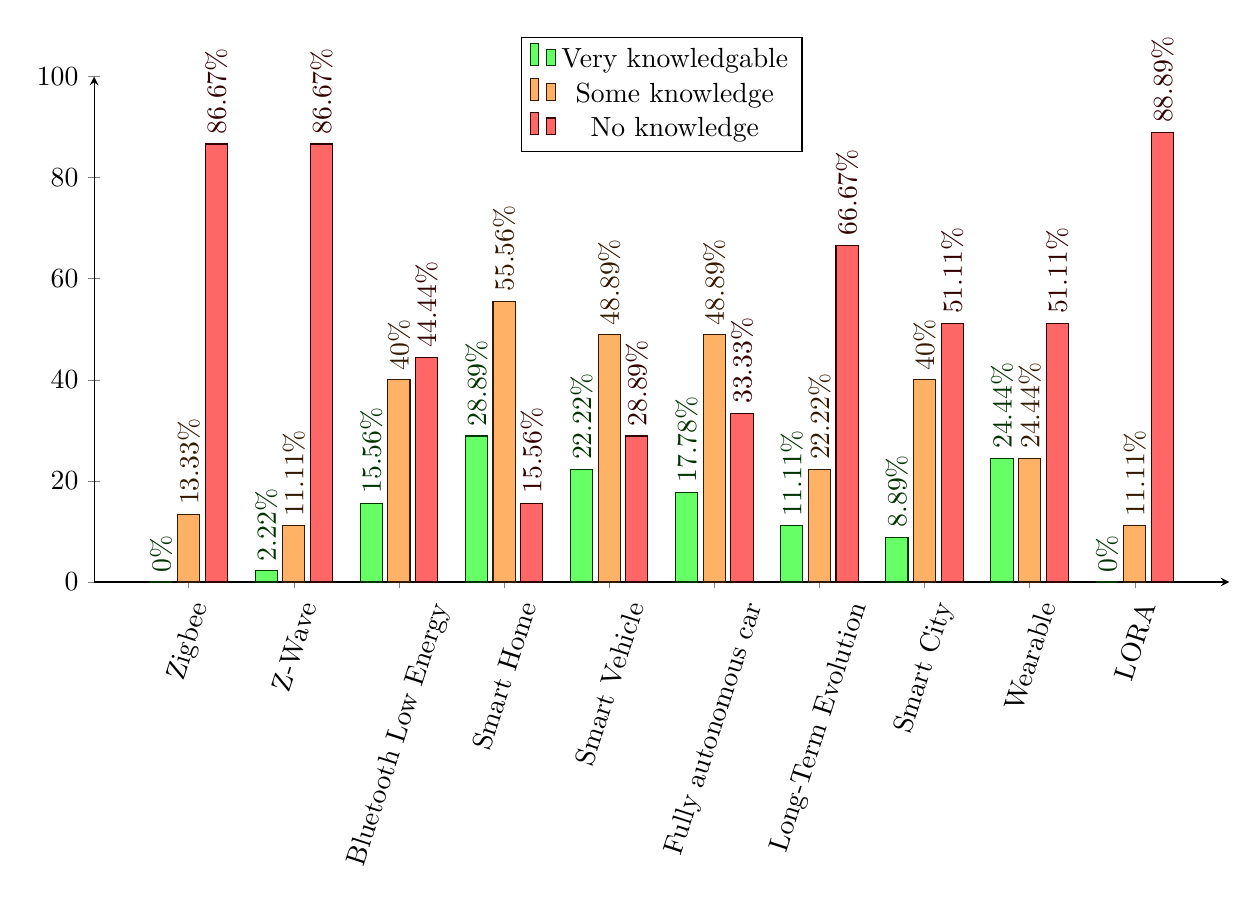
\begin{tikzpicture}
    \begin{axis}[
        height=8cm,
        width=16cm,
        symbolic x coords={Zigbee, Z-Wave,Bluetooth Low Energy,Smart Home,Smart Vehicle,Fully autonomous car,Long-Term Evolution,Smart City,Wearable,LORA},
        ybar,
        bar width=8pt,
        ymin=0,
        ymax=100,
        xticklabel style={rotate=72},
        axis x line=bottom,
        axis y line=left,
        enlarge x limits=0.1,
        nodes near coords={\pgfmathprintnumber\pgfplotspointmeta\%},
        every node near coord/.append style={rotate=90, anchor=west},
        legend style={at={(0.5,0.85)},anchor=south}
    ]
        \addplot[green!20!black,fill=green!60!white] coordinates {(Zigbee,0) (Z-Wave,2.22) (Bluetooth Low Energy,15.56) (Smart Home,28.89) (Smart Vehicle,22.22) (Fully autonomous car,17.78) (Long-Term Evolution,11.11) (Smart City,8.89) (Wearable,24.44) (LORA,0)};
        \addlegendentry{Very knowledgable}
        \addplot[orange!20!black,fill=orange!60!white] coordinates {(Zigbee,13.33) (Z-Wave,11.11) (Bluetooth Low Energy,40) (Smart Home,55.56) (Smart Vehicle,48.89) (Fully autonomous car,48.89) (Long-Term Evolution,22.22) (Smart City,40) (Wearable,24.44) (LORA,11.11)};
        \addlegendentry{Some knowledge}
        \addplot[red!20!black,fill=red!60!white] coordinates {(Zigbee,86.67) (Z-Wave,86.67) (Bluetooth Low Energy,44.44) (Smart Home,15.56) (Smart Vehicle,28.89) (Fully autonomous car,33.33) (Long-Term Evolution,66.67) (Smart City,51.11) (Wearable,51.11) (LORA,88.89)};
        \addlegendentry{No knowledge}
    \end{axis}
\end{tikzpicture}
\end{document}
